\documentclass[12pt]{article}
% \documentclass[12pt,oneside,a4paper]{article}
\usepackage[utf8]{inputenc}
\usepackage[english ]{babel}
\usepackage[sc]{mathpazo}
\linespread{1.05}         
\usepackage[T1]{fontenc}
\usepackage{xcolor}
\definecolor{aaublue}{RGB}{33,26,82}% dark blue
\usepackage{graphicx}
\usepackage{array,booktabs}
\usepackage{framed}
\usepackage{epstopdf}
\usepackage[normalem]{ulem}
\usepackage{amsmath, amssymb}
\usepackage[framed,amsthm, amsmath,thmmarks]{ntheorem}
\usepackage[left = 1in, right=1in, top = 1in, bottom = 1in ]{geometry}
\usepackage{lastpage}
\usepackage{mathrsfs}
\usepackage{amsbsy,bm}
\usepackage{multirow}
\usepackage{patchcmd}
\usepackage{comment}
\usepackage{algorithm}
\usepackage{algpseudocode}
\usepackage{subcaption} %for subfigures. 
\usepackage{lipsum}
\usepackage{caption}
\newtheorem{proposition}{Proposition}[section]
\newtheorem{definition}{Definition}
\newtheorem{example}{Example}
\newtheorem{exercise}{Exercise}
\newtheorem{theorem}{Theorem}
%================================================================
\usepackage[utf8]{inputenc}
\usepackage[english ]{babel}
\usepackage[sc]{mathpazo}
\linespread{1.05}         
\usepackage[T1]{fontenc}
%================================================================
\usepackage[utf8]{inputenc}
%================================================================
\usepackage[utf8]{inputenc}

\captionsetup{%
  font=footnotesize,% set font size to footnotesize
  %labelfont=bf % bold label (e.g., Figure 3.2) font
}

\usepackage[left = 1in, right=1in, top = 1in, bottom = 1in ]{geometry}
% \usepackage{titlesec}

\usepackage{fancyhdr}
\fancyhf{} 
% \renewcommand{\headrulewidth}{0pt} %remove the horizontal line in the header
% \fancyhead[LO]{\small\nouppercase\rightmark} %uneven page - section title
% \raggedbottom

\usepackage{calc}
\usepackage[numbers]{natbib}
\usepackage[nottoc]{tocbibind}
\usepackage{lastpage}
\setlength{\marginparwidth}{2cm}
\usepackage[
   colorinlistoftodos, %enable a coloured square in the list of todos
   textwidth=\marginparwidth, %set the width of the todonotes
   textsize=scriptsize, %size of the text in the todonotes
   ]{todonotes}
\usepackage{hyperref}
\hypersetup{hidelinks}
\usepackage[noabbrev,capitalise]{cleveref}
\usepackage{mathrsfs}
\usepackage{amsbsy,bm}
% \usepackage{subcaption}
% \usepackage{multirow}
\usepackage{algorithm}
\usepackage{patchcmd}
% \usepackage{algorithmic}
\usepackage{comment}
\newcommand{\dt}{\Delta t}
\newcommand{\D}{\Delta}
\newcommand{\abs}[1]{\left| #1  \right|}
\newcommand{\R}{\mathbb{R}}
\newcommand{\eps}{\varepsilon}
\newcommand{\bx}{\boldsymbol x}
\usepackage[utf8]{inputenc}
\usepackage[english]{babel}
\usepackage{bbm}

%%%%%%%%%%%%%%%%%%%%%%%%%%%%%%%%%%%%%%%%%%%%%%%
\usepackage{setspace}
\usepackage{pgfplots}
\usepackage{cancel}
\usepackage{longtable}

%====================================================================
\begin{document}
\doublespacing
%====================================================================
\newcommand{\HRule}[1]{\rule{\linewidth}{#1}}   % Horizontal rule

\makeatletter             % Title
\def\printtitle{%           
    {\centering \@title\par}}
\makeatother                  

\makeatletter             % Author
\def\printauthor{%          
    {\centering \large \@author}}       
\makeatother              

% --------------------------------------------------------------------
% Metadata (Change this)
% --------------------------------------------------------------------
\title{ \normalsize \textsc{Lecture Notes}  % Subtitle
      \\[2.0cm]               % 2cm spacing
      \HRule{0.5pt} \\            % Upper rule
      \LARGE \textbf{\uppercase{MAT 251 \\
      Brief Calculus}}  % Title
      \HRule{2pt} \\ [0.5cm]    % Lower rule + 0.5cm spacing
      \normalsize \today      % Todays date
    }

\author{
    \textbf{Atta Ullah, PhD}\\
    College of Humanity and Social Sciences \\  
    Grand Canyon University, Phoenix Arizona \\
}


% ------------------------------------------------------------------------------
% Maketitle
% ------------------------------------------------------------------------------
\thispagestyle{empty}   % Remove page numbering on this page

\printtitle         % Print the title data as defined above
    \vfill
\printauthor        % Print the author data as defined above
\clearpage
% ------------------------------------------------------------------------------
% Begin document
% ------------------------------------------------------------------------------

\tableofcontents
\clearpage
%=====================================================================
\newpage

\section{Equation of a Line in Slope-Intercept Form}

The equation of a straight line can be expressed in various forms. One of the most commonly used forms is the \textit{slope-intercept form}. This form is useful because it provides direct information about the slope and the y-intercept of the line.

\begin{definition}[Slope-Intercept Form]
The slope-intercept form of the equation of a line is given by:

\[
y = mx + b
\]

where:
\begin{itemize}
    \item \( y \) is the dependent variable (the value of the output),
    \item \( x \) is the independent variable (the value of the input),
    \item \( m \) is the slope of the line, which represents the rate of change of \( y \) with respect to \( x \),
    \item \( b \) is the y-intercept, which is the value of \( y \) when \( x = 0 \).
\end{itemize}
\end{definition}

\begin{definition}[Slope \( m \)]

The slope \( m \) is a measure of how steep the line is. It is calculated as the ratio of the change in \( y \) (the vertical change) to the change in \( x \) (the horizontal change) between two points on the line:

\[
m = \frac{\Delta y}{\Delta x} = \frac{y_2 - y_1}{x_2 - x_1}
\]
\end{definition}

This means that for every unit increase in \( x \), the value of \( y \) changes by \( m \) units.

\begin{definition} [Y-Intercept (\( b \))]
The y-intercept \( b \) is the point where the line crosses the y-axis. It is the value of \( y \) when \( x = 0 \). In the equation \( y = mx + b \), if we substitute \( x = 0 \), we get:

\[
y = m(0) + b \quad \Rightarrow \quad y = b
\]

Thus, the y-intercept is the value of \( y \) when the line intersects the y-axis.
\end{definition}

\begin{example}

Consider the equation:

\[
y = 2x + 3
\]

In this equation:
\begin{itemize}
    \item The slope \( m = 2 \), which means that for every unit increase in \( x \), \( y \) increases by 2 units.
    \item The y-intercept \( b = 3 \), which means the line crosses the y-axis at \( y = 3 \).
\end{itemize}

This is a line with a slope of 2 and a y-intercept of 3. The graph of this line is shown below:

\begin{center}
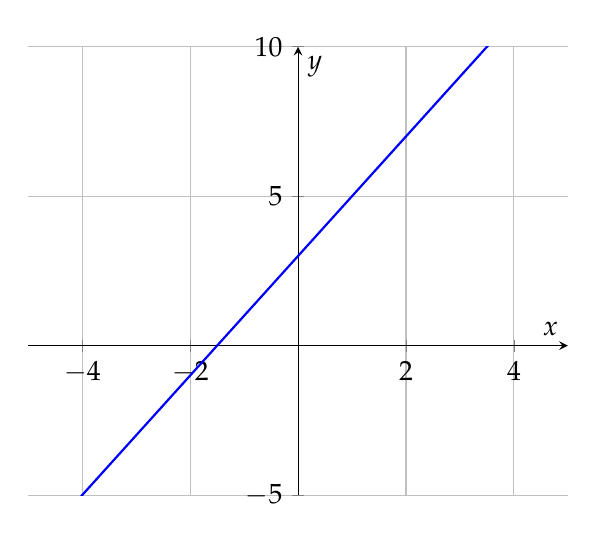
\begin{tikzpicture}
\begin{axis}[
    axis lines = middle, 
    xlabel = \( x \),
    ylabel = \( y \),
    xmin=-5, xmax=5, ymin=-5, ymax=10,
    grid = both,
    domain=-5:5,
    samples=100]
    \addplot[blue, thick] {2*x + 3};
\end{axis}
\end{tikzpicture}
\end{center}
\end{example}

\subsection{Three Cases for Finding the Equation of a Line}

We now discuss three different cases where you may need to find the equation of a line:

\subsubsection{Case 1: When Two Points Are Given}
If two points \((x_1, y_1)\) and \((x_2, y_2)\) are given, the equation of the line can be found in the following steps:

1. Find the slope \( m \) using the formula:
   \[
   m = \frac{y_2 - y_1}{x_2 - x_1}
   \]
2. Use the slope \( m \) and one of the points, say \((x_1, y_1)\), to find the y-intercept \( b \) by substituting into the equation \( y = mx + b \).

3. The final equation of the line will be:
   \[
   y = mx + b
   \]

\begin{example}
 Given points \((1, 2)\) and \((3, 6)\), find the equation of the line.

1. Calculate the slope:
   \[
   m = \frac{6 - 2}{3 - 1} = \frac{4}{2} = 2
   \]

2. Use the point \((1, 2)\) to find \( b \):
   \[
   2 = 2(1) + b \quad \Rightarrow \quad b = 0
   \]

3. The equation of the line is:
   \[
   y = 2x
   \]

\end{example}
\subsubsection{Case 2: When the Slope and a Point Are Given}
If the slope \( m \) and a point \((x_1, y_1)\) are given, you can use the point-slope form of the equation of a line, which is:

\[
y - y_1 = m(x - x_1)
\]

Then, solve for \( y \) to get the equation in slope-intercept form:

\[
y = m(x - x_1) + y_1
\]

\begin{example}

 Given slope \( m = 3 \) and the point \((2, 4)\), find the equation of the line.

1. Use the point-slope form:
   \[
   y - 4 = 3(x - 2)
   \]

2. Simplify to get the slope-intercept form:
   \[
   y = 3x - 6 + 4 \quad \Rightarrow \quad y = 3x - 2
   \]

\end{example}

\subsubsection{Case 3: When the Y-Intercept and a Point Are Given}
If the y-intercept \( b \) and a point \((x_1, y_1)\) are given, the equation of the line can be directly written as:

\[
y = mx + b
\]

To find the slope \( m \), use the given point \((x_1, y_1)\) and substitute into the equation:

\[
m = \frac{y_1 - b}{x_1}
\]

Then, the equation becomes:
\[
y = mx + b
\]

\begin{example}

 Given \( b = 5 \) and the point \((2, 9)\), find the equation of the line.

1. Calculate the slope:
   \[
   m = \frac{9 - 5}{2} = \frac{4}{2} = 2
   \]

2. The equation of the line is:
   \[
   y = 2x + 5
   \]

\end{example}


% %%%%%%%%%%%%%%%%%%%%%%%%%%%%%%%%%%%%%%%%

\subsection{Graphing Linear Equations}

Here we will graph the following linear equations:
\begin{itemize}
    \item \( 2x - y = 4 \)
    \item \( 3x - 4y = 4 \)
    \item \( y = 2 \)
    \item \( x = 3 \)
\end{itemize}

We will graph each of these equations on the same coordinate plane.

\subsubsection*{Graph of \( 2x - y = 4 \)}

Rearrange the equation into slope-intercept form \( y = mx + b \) to make it easier to plot:

\[
2x - y = 4 \quad \Rightarrow \quad y = 2x - 4
\]

This is a line with slope \( m = 2 \) and y-intercept \( b = -4 \).

\begin{center}
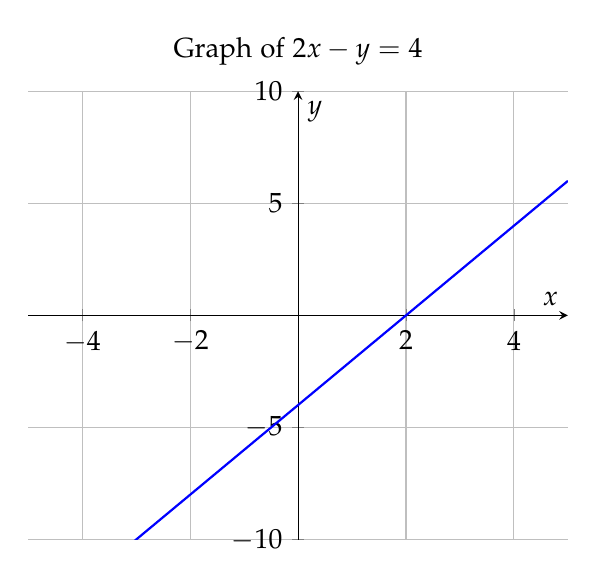
\begin{tikzpicture}
\begin{axis}[
    axis lines = middle,
    xlabel = \( x \), ylabel = \( y \),
    grid = both, 
    xmin=-5, xmax=5, ymin=-10, ymax=10,
    title = {Graph of \( 2x - y = 4 \)}
]
    \addplot[blue, thick] {2*x - 4};
\end{axis}
\end{tikzpicture}
\end{center}

\subsubsection*{Graph of \( 3x - 4y = 4 \)}

Rearrange the equation into slope-intercept form:

\[
3x - 4y = 4 \quad \Rightarrow \quad 4y = 3x - 4 \quad \Rightarrow \quad y = \frac{3}{4}x - 1
\]

This is a line with slope \( m = \frac{3}{4} \) and y-intercept \( b = -1 \).

\begin{center}
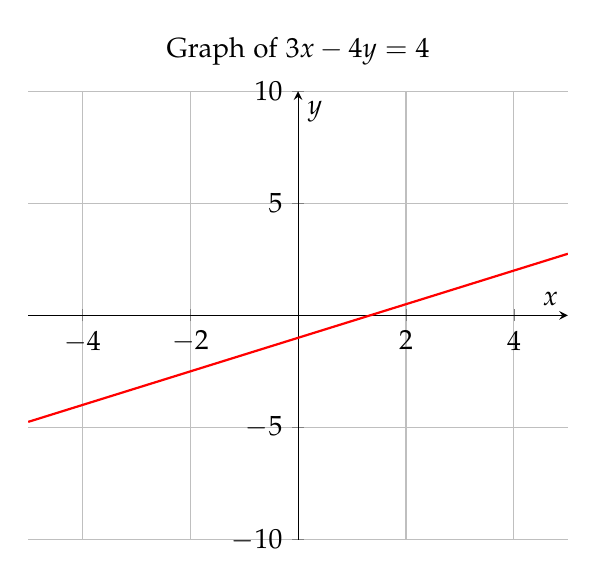
\begin{tikzpicture}
\begin{axis}[
    axis lines = middle,
    xlabel = \( x \), ylabel = \( y \),
    grid = both, 
    xmin=-5, xmax=5, ymin=-10, ymax=10,
    title = {Graph of \( 3x - 4y = 4 \)}
]
    \addplot[red, thick] {3/4*x - 1};
\end{axis}
\end{tikzpicture}
\end{center}

\subsubsection*{Graph of \( y = 2 \)}

This is a horizontal line at \( y = 2 \).

\begin{center}
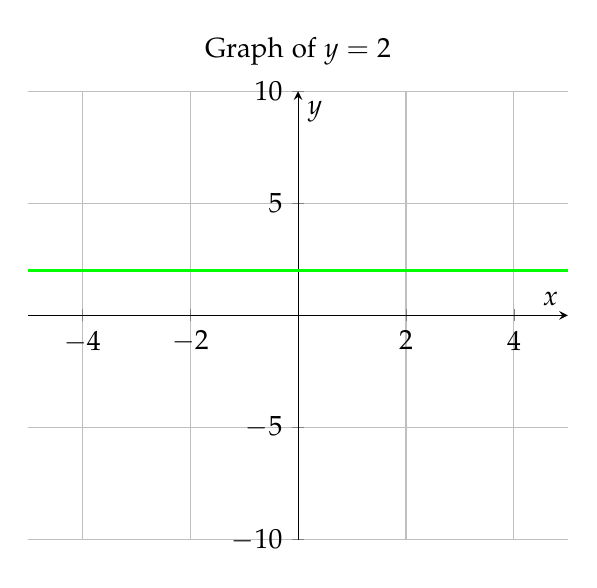
\begin{tikzpicture}
\begin{axis}[
    axis lines = middle,
    xlabel = \( x \), ylabel = \( y \),
    grid = both, 
    xmin=-5, xmax=5, ymin=-10, ymax=10,
    title = {Graph of \( y = 2 \)}
]
    \addplot[green, thick, domain=-5:5] {2};
\end{axis}
\end{tikzpicture}
\end{center}

\subsection*{Graph of \( x = 3 \)}

This is a vertical line at \( x = 3 \).

\begin{center}
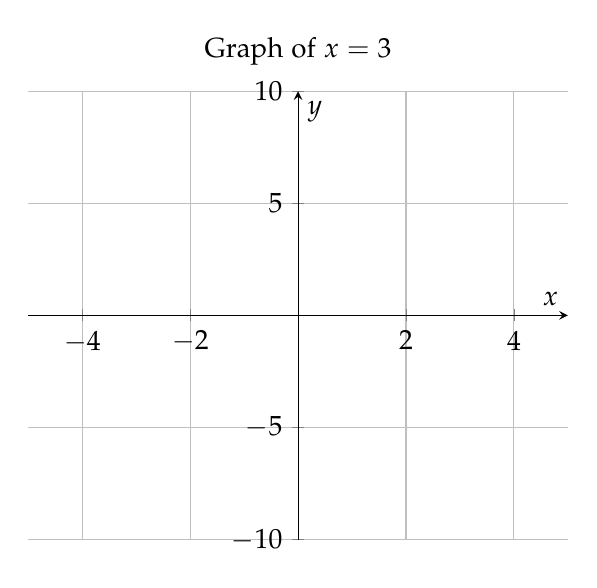
\begin{tikzpicture}
\begin{axis}[
    axis lines = middle,
    xlabel = \( x \), ylabel = \( y \),
    grid = both, 
    xmin=-5, xmax=5, ymin=-10, ymax=10,
    title = {Graph of \( x = 3 \)}
]
    % \addplot[orange, thick, domain=-10:10] {3};
\end{axis}
\end{tikzpicture}
\end{center}
%%%
We will now find the slope of the line given by the equation \( 2x - 3y = 12 \), and also evaluate the slope at a specific point, \( (x = -3, y = 1) \).

\subsection*{Finding the Slope of the Line \( 2x - 3y = 12 \)}

To find the slope of the line, we first need to rewrite the equation \( 2x - 3y = 12 \) in slope-intercept form, which is:

\[
y = mx + b
\]

where \( m \) is the slope of the line and \( b \) is the y-intercept. We begin by isolating \( y \).

Starting with the equation:

\[
2x - 3y = 12
\]

Subtract \( 2x \) from both sides:

\[
-3y = -2x + 12
\]

Now, divide through by \( -3 \) to solve for \( y \):

\[
y = \frac{2}{3}x - 4
\]

From this equation, we can see that the slope \( m \) is:

\[
m = \frac{2}{3}
\]

Thus, the slope of the line is \( \frac{2}{3} \).


\subsection*{Slope at a Specific Point}

Next, we are asked to find the slope at the point \( (x = -3, y = 1) \). However, the slope of a straight line is constant, meaning it does not depend on the specific point. Since the equation \( 2x - 3y = 12 \) represents a straight line, the slope at any point on this line is the same.

Therefore, the slope at the point \( (x = -3, y = 1) \) is the same as the slope of the line, which is:

\[
m = \frac{2}{3}
\]


The slope of the line given by the equation \( 2x - 3y = 12 \) is \( \frac{2}{3} \), and the slope at the point \( (x = -3, y = 1) \) is also \( \frac{2}{3} \).

%%%
\section{Functions}

\subsection{Functions Evaluation}

The process of evaluating a function involves substituting specific values for the independent variable \( x \) into the function's expression and calculating the resulting output. If \( f(x) \) is a function, the value of the function at a specific point \( x = a \) is denoted as \( f(a) \), and is computed by substituting \( x = a \) into the expression for \( f(x) \).

To evaluate a function \( f(x) \) at a specific value \( x = a \):
\begin{enumerate}
    \item Substitute the given value of \( x \) into the expression for \( f(x) \).
    \item Simplify the expression, if necessary, to find the value of the function at that point.
\end{enumerate}

For example, if \( f(x) = 2x + 3 \), and we want to evaluate the function at \( x = 4 \), we substitute \( x = 4 \) into the expression:
\[
f(4) = 2(4) + 3 = 8 + 3 = 11
\]
Thus, \( f(4) = 11 \).


\subsection*{Evaluating Functions \( f(x) = \frac{1}{x+1} \)}

Consider the function:
\[
f(x) = \frac{1}{x+1}
\]

Now, perform the following evaluations:

\begin{enumerate}
    \item \textbf{Find \( f(0) \):}
    \[
    f(0) = \frac{1}{0 + 1} = \frac{1}{1} = 1
    \]
    Therefore, \( f(0) = 1 \).
    
    \item \textbf{Find \( f(-1) \):}
    \[
    f(-1) = \frac{1}{-1 + 1} = \frac{1}{0}
    \]

    \item \textbf{Find \( f(t) \):}
    \[
    f(t) = \frac{1}{t + 1}
    \]

    \item \textbf{Find \( f(x + h) \):}
    \[
    f(x + h) = \frac{1}{(x + h) + 1} = \frac{1}{x + h + 1}
    \]

    \item \textbf{Find \( \frac{f(x + h) - f(x)}{h} \):}
    First, we need to find \( f(x + h) \) and \( f(x) \).
    \[
    f(x + h) = \frac{1}{x + h + 1}, \quad f(x) = \frac{1}{x + 1}
    \]
    Now, we compute the difference:
    \[
    f(x + h) - f(x) = \frac{1}{x + h + 1} - \frac{1}{x + 1}
    \]
    To subtract these fractions, we need a common denominator:
    \[
    f(x + h) - f(x) = \frac{(x + 1) - (x + h + 1)}{(x + h + 1)(x + 1)} = \frac{(x + 1) - (x + 1 + h)}{(x + h + 1)(x + 1)} = \frac{-h}{(x + h + 1)(x + 1)}
    \]
    Now, divide by \( h \):
    \[
    \frac{f(x + h) - f(x)}{h} = \frac{-h}{h(x + h + 1)(x + 1)} = \frac{-1}{(x + h + 1)(x + 1)}
    \]
    Therefore, the difference quotient is:
    \[
    \frac{f(x + h) - f(x)}{h} = \frac{-1}{(x + h + 1)(x + 1)}
    \]
\end{enumerate}

% %%%%%%%%%%%%%%%%%%%%%%%%%%%%%%%%
\subsection{Definitions}

\begin{definition}[Function]

A function is a relation between a set of inputs (the domain) and a set of possible outputs (the range), such that each input is related to exactly one output. In other words, for every \( x \) in the domain, there exists a unique corresponding \( y \) in the range.

\end{definition}



\begin{definition}
[Domain of a Function]

The domain of a function is the set of all possible input values (usually denoted \( x \)) that will produce a valid output. The domain may be restricted by various factors, such as division by zero or the need for the input to be a real number.
\end{definition}

\begin{example}

%%%%%%%%%%%%%%%%%%%%%%%%%%%%%%%%%%%%%%%%%%%%
%%%%%%%%%%%%%%%%%%%%%%%%%%%%%%%%%%%%%%%%%%%%

Find the domain for following functions: 
\begin{itemize}
\item \( f(x) = \sqrt{9 - x^2}\)
\item \( f(x) = \frac{1}{16 - x^2}\) 
\item \( f(x) = \sqrt{\frac{5}{x^2 - 36}}\) 
\end{itemize}

\end{example}

\subsubsection*{Solution:}


\textbf{Domain of \( f(x) = \sqrt{9 - x^2} \)}

For a square root function, the expression inside the square root must be non-negative for the function to be defined. Therefore, we need:
\[
9 - x^2 \geq 0.
\]

Solving this inequality:
\[
9 \geq x^2 \quad \Rightarrow \quad -3 \leq x \leq 3.
\]

Thus, the domain of \( f(x) = \sqrt{9 - x^2} \) is:
\[
\boxed{[-3, 3]}.
\]

\textbf{Domain of \( f(x) = \frac{1}{16 - x^2} \)}

For a rational function, the denominator must not be zero. Therefore, we need to find the values of \( x \) for which the denominator is not zero. We set the denominator equal to zero and solve for \( x \):
\[
16 - x^2 = 0 \quad \Rightarrow \quad x^2 = 16 \quad \Rightarrow \quad x = \pm 4.
\]

Therefore, the domain of \( f(x) = \frac{1}{16 - x^2} \) is all real numbers except \( x = 4 \) and \( x = -4 \). In interval notation, the domain is:
\[
\boxed{(-\infty, -4) \cup (-4, 4) \cup (4, \infty)}.
\]

\textbf{Domain of \( f(x) = \sqrt{\frac{5}{x^2 - 36}} \)}

For a square root function, the expression inside the square root must be non-negative. Additionally, the denominator must not be zero. Therefore, we need to find the values of \( x \) such that:
\[
\frac{5}{x^2 - 36} \geq 0 \quad \text{and} \quad x^2 - 36 \neq 0.
\]

First, solve for when the denominator is zero:
\[
x^2 - 36 = 0 \quad \Rightarrow \quad x^2 = 36 \quad \Rightarrow \quad x = \pm 6.
\]
Thus, \( x = \pm 6 \) must be excluded from the domain.

Next, solve the inequality:
\[
x^2 - 36 > 0.
\]
This inequality holds when:
\[
x > 6 \quad \text{or} \quad x < -6.
\]

Therefore, the domain of \( f(x) = \sqrt{\frac{5}{x^2 - 36}} \) is:
\[
\boxed{(-\infty, -6) \cup (6, \infty)}.
\]


%%%%%%%%%%%%%%%%%%%%%%%%%%%%%%%%%%%%%%%%%%%%
%%%%%%%%%%%%%%%%%%%%%%%%%%%%%%%%%%%%%%%%%%%%

\begin{definition}
[ange of a Function]

The range of a function is the set of all possible output values (usually denoted \( y \)) that the function can produce. This depends on the form of the function and the restrictions on its domain.

\end{definition}

\subsection{The Vertical Line Test}

The vertical line test is a method used to determine whether a graph represents a function. The test states that:
\begin{itemize}
    \item If any vertical line intersects the graph of a relation at more than one point, then the relation is not a function.
    \item If every vertical line intersects the graph at most once, then the relation is a function.
\end{itemize}

This test helps to identify whether the graph represents a function, as it ensures that for each \( x \)-value (input), there is only one \( y \)-value (output).


To better understand these concepts, we can look at some graphs that demonstrate the vertical line test and the domain and range.

\subsection*{Example 1: A Function}

Consider the function \( f(x) = x^2 \), which is a parabola. Let's graph it and apply the vertical line test.

\begin{center}
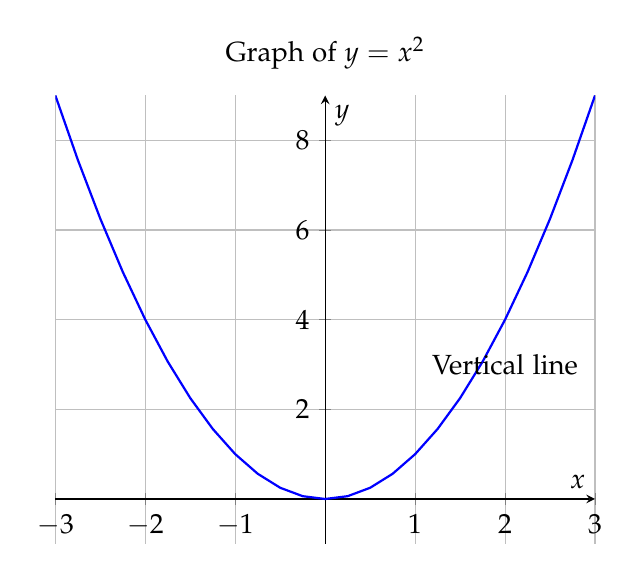
\begin{tikzpicture}
\begin{axis}[
    axis lines = middle, 
    xlabel = \( x \), ylabel = \( y \),
    grid = both, 
    xmin=-3, xmax=3, ymin=-1, ymax=9,
    title = {Graph of \( y = x^2 \)},
    domain=-3:3
]
    \addplot[blue, thick] {x^2};
    % Vertical line for test
    % \addplot[red, thick, domain=-3:3] {4};
    \node at (axis cs:2,3) {Vertical line};
\end{axis}
\end{tikzpicture}
\end{center}

In the above graph of \( f(x) = x^2 \), every vertical line intersects the graph at exactly one point, thus passing the vertical line test. Therefore, this graph represents a function.

\subsection*{Example 2: Not a Function}

Now, consider the graph of the relation \( y^2 = x \), which is a sideways parabola. We will apply the vertical line test to this graph.

\begin{center}
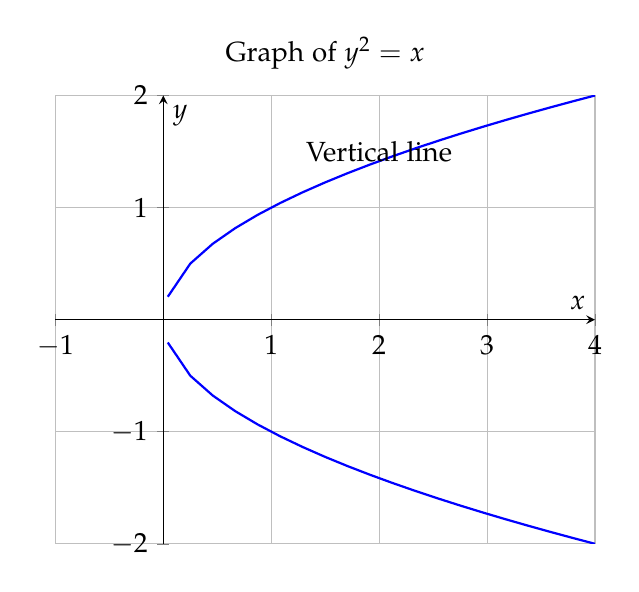
\begin{tikzpicture}
\begin{axis}[
    axis lines = middle, 
    xlabel = \( x \), ylabel = \( y \),
    grid = both, 
    xmin=-1, xmax=4, ymin=-2, ymax=2,
    title = {Graph of \( y^2 = x \)},
    domain=-1:4
]
    \addplot[blue, thick] {sqrt(x)};
    \addplot[blue, thick] {-sqrt(x)};
    % Vertical line for test
    % \addplot[red, thick, domain=-1:4] {1};
    \node at (axis cs:2,1.5) {Vertical line};
\end{axis}
\end{tikzpicture}
\end{center}

In the graph of \( y^2 = x \), a vertical line intersects the graph at two points, which means this relation does not pass the vertical line test and is \textit{not} a function.

%%%%%%%%%%%%%%%%%%%%%
Functions can be classified as \textit{even} or \textit{odd} based on their symmetry properties. Understanding whether a function is even or odd can help in graphing, analyzing, and solving various mathematical problems. 

\section{Even and Odd Functions}

\begin{definition}[Even Functions]

A function \( f(x) \) is called \textit{even} if its graph is symmetric about the y-axis. Mathematically, a function \( f(x) \) is even if for all \( x \) in the domain of \( f \), the following condition holds:

\[
f(-x) = f(x)
\]
\end{definition}

\subsection{Properties of Even Functions}
\begin{itemize}
    \item The graph of an even function is symmetric about the y-axis.
    \item If a function is even, it satisfies the equation \( f(-x) = f(x) \) for all values of \( x \) in its domain.
    \item The sum or difference of two even functions is also an even function.
    \item The product of two even functions is also an even function.
\end{itemize}

\subsection*{Example of an Even Function}

An example of an even function is the quadratic function \( f(x) = x^2 \). Let’s check if this function is even by verifying whether \( f(-x) = f(x) \):

\[
f(-x) = (-x)^2 = x^2 = f(x)
\]

Since \( f(-x) = f(x) \), the function \( f(x) = x^2 \) is an even function.

\subsection*{Graph of \( f(x) = x^2 \)}

Below is the graph of \( f(x) = x^2 \), which is symmetric about the y-axis.

\begin{center}
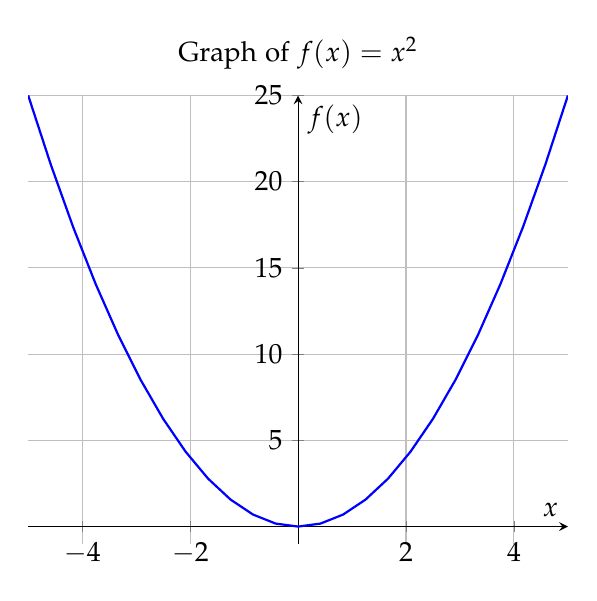
\begin{tikzpicture}
\begin{axis}[
    axis lines = middle, 
    xlabel = \( x \), ylabel = \( f(x) \),
    grid = both, 
    xmin=-5, xmax=5, ymin=-1, ymax=25,
    title = {Graph of \( f(x) = x^2 \)}
]
    \addplot[blue, thick] {x^2};
\end{axis}
\end{tikzpicture}
\end{center}

\begin{definition}
[Odd Functions]
A function \( f(x) \) is called \textit{odd} if its graph is symmetric about the origin. Mathematically, a function \( f(x) \) is odd if for all \( x \) in the domain of \( f \), the following condition holds:

\[
f(-x) = -f(x)
\]

\end{definition}
\subsection{Properties of Odd Functions}
\begin{itemize}
    \item The graph of an odd function is symmetric about the origin.
    \item If a function is odd, it satisfies the equation \( f(-x) = -f(x) \) for all values of \( x \) in its domain.
    \item The sum or difference of two odd functions is also an odd function.
    \item The product of an odd function and an even function is an odd function.
\end{itemize}

\subsection*{Example of an Odd Function}

An example of an odd function is the cubic function \( f(x) = x^3 \). Let’s check if this function is odd by verifying whether \( f(-x) = -f(x) \):

\[
f(-x) = (-x)^3 = -x^3 = -f(x)
\]

Since \( f(-x) = -f(x) \), the function \( f(x) = x^3 \) is an odd function.

\subsection*{Graph of \( f(x) = x^3 \)}

Below is the graph of \( f(x) = x^3 \), which is symmetric about the origin.

\begin{center}
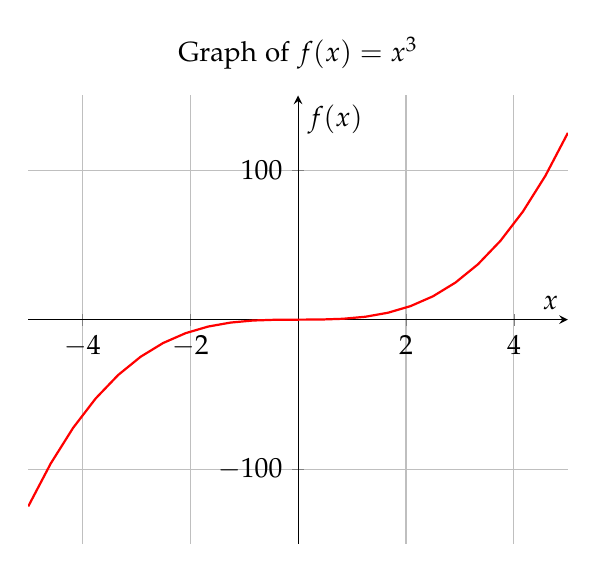
\begin{tikzpicture}
\begin{axis}[
    axis lines = middle, 
    xlabel = \( x \), ylabel = \( f(x) \),
    grid = both, 
    xmin=-5, xmax=5, ymin=-150, ymax=150,
    title = {Graph of \( f(x) = x^3 \)}
]
    \addplot[red, thick] {x^3};
\end{axis}
\end{tikzpicture}
\end{center}


\begin{itemize}
    \item A function is \textit{even} if \( f(-x) = f(x) \) for all \( x \) in its domain. The graph is symmetric about the y-axis.
    \item A function is \textit{odd} if \( f(-x) = -f(x) \) for all \( x \) in its domain. The graph is symmetric about the origin.
\end{itemize}



\subsection{Graphs of Common Functions}

This part contains the graphs of the following functions:
\begin{itemize}
    \item \( f(x) = x \)
    \item \( f(x) = x^2 \)
    \item \( f(x) = x^3 \)
    \item \( f(x) = |x| \)
    \item \( f(x) = \sqrt{x} \)
    \item \( f(x) = \frac{1}{x} \)
    \item \( f(x) = \frac{1}{|x|^2} \)
\end{itemize}


\subsubsection*{Graph of \( f(x) = x \)}

The graph of the function \( f(x) = x \) is a straight line passing through the origin with a slope of 1.

\begin{center}
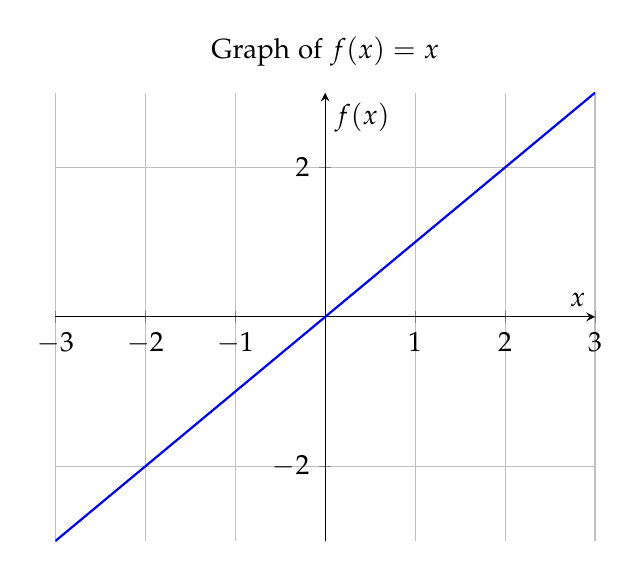
\begin{tikzpicture}
\begin{axis}[
    axis lines = middle,
    xlabel = \( x \),
    ylabel = \( f(x) \),
    grid = both,
    xmin=-3, xmax=3, ymin=-3, ymax=3,
    title = {Graph of \( f(x) = x \)}
]
    \addplot[blue, thick] {x};
\end{axis}
\end{tikzpicture}
\end{center}

\subsubsection*{Graph of \( f(x) = x^2 \)}

The graph of \( f(x) = x^2 \) is a parabola opening upwards.

\begin{center}
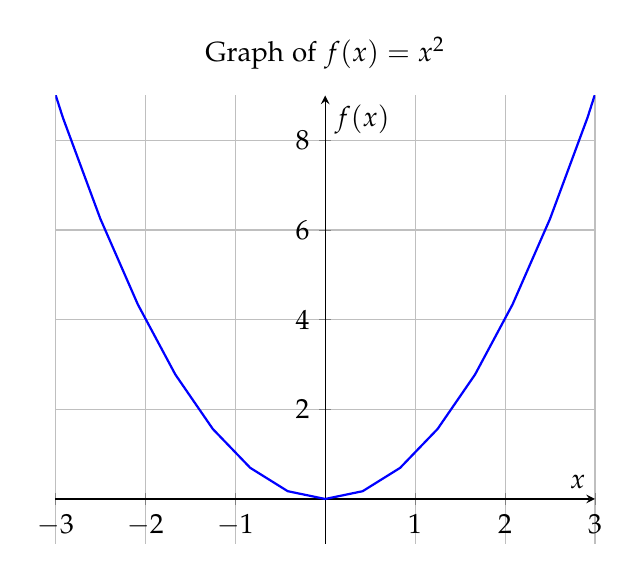
\begin{tikzpicture}
\begin{axis}[
    axis lines = middle,
    xlabel = \( x \),
    ylabel = \( f(x) \),
    grid = both,
    xmin=-3, xmax=3, ymin=-1, ymax=9,
    title = {Graph of \( f(x) = x^2 \)}
]
    \addplot[blue, thick] {x^2};
\end{axis}
\end{tikzpicture}
\end{center}

\subsection*{Graph of \( f(x) = x^3 \)}

The graph of \( f(x) = x^3 \) is an odd function with symmetric behavior about the origin.

\begin{center}
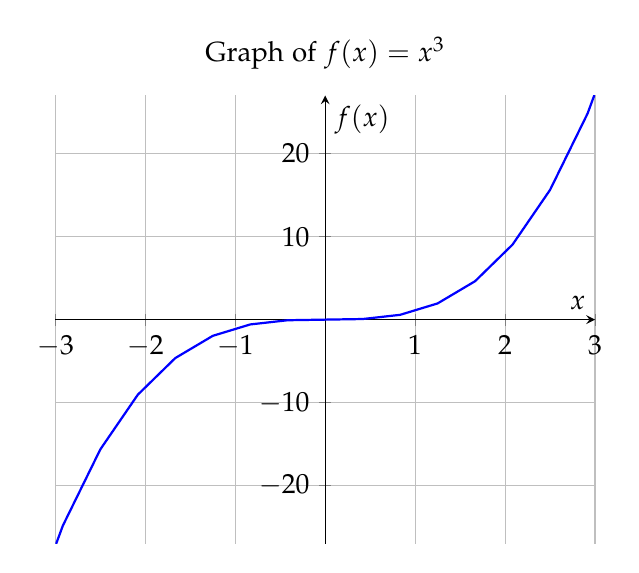
\begin{tikzpicture}
\begin{axis}[
    axis lines = middle,
    xlabel = \( x \),
    ylabel = \( f(x) \),
    grid = both,
    xmin=-3, xmax=3, ymin=-27, ymax=27,
    title = {Graph of \( f(x) = x^3 \)}
]
    \addplot[blue, thick] {x^3};
\end{axis}
\end{tikzpicture}
\end{center}

\subsection*{Graph of \( f(x) = |x| \)}

The graph of \( f(x) = |x| \) is a "V"-shaped graph, representing the absolute value function.

\begin{center}
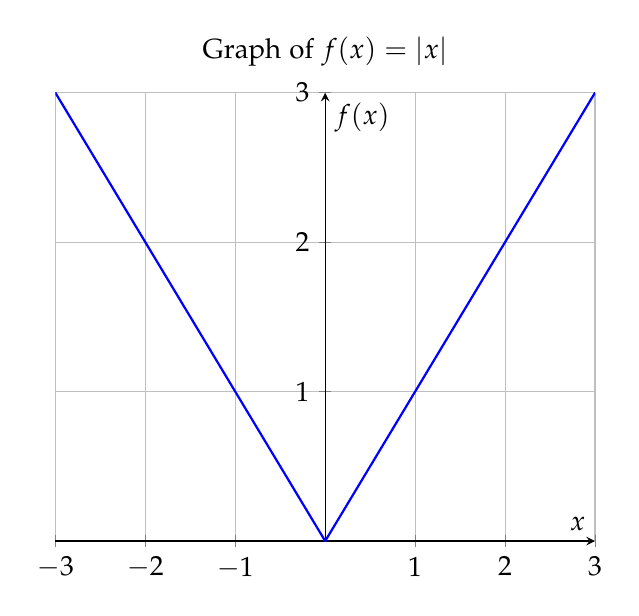
\begin{tikzpicture}
\begin{axis}[
    axis lines = middle,
    xlabel = \( x \),
    ylabel = \( f(x) \),
    grid = both,
    xmin=-3, xmax=3, ymin=0, ymax=3,
    title = {Graph of \( f(x) = |x| \)}
]
    \addplot[blue, thick] {abs(x)};
\end{axis}
\end{tikzpicture}
\end{center}

\subsection*{Graph of \( f(x) = \sqrt{x} \)}

The graph of \( f(x) = \sqrt{x} \) is a curve that only exists for \( x \geq 0 \).

\begin{center}
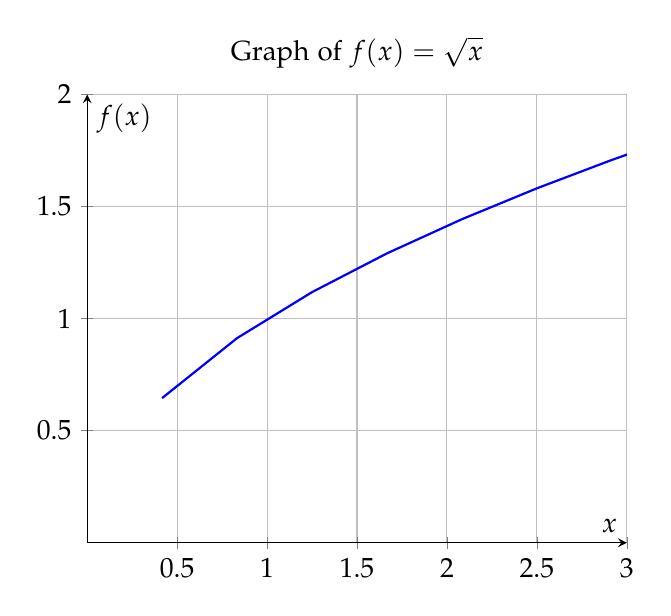
\begin{tikzpicture}
\begin{axis}[
    axis lines = middle,
    xlabel = \( x \),
    ylabel = \( f(x) \),
    grid = both,
    xmin=0, xmax=3, ymin=0, ymax=2,
    title = {Graph of \( f(x) = \sqrt{x} \)}
]
    \addplot[blue, thick] {sqrt(x)};
\end{axis}
\end{tikzpicture}
\end{center}

\subsection*{Graph of \( f(x) = \frac{1}{x} \)}

The graph of \( f(x) = \frac{1}{x} \) has two asymptotes: one at \( x = 0 \) and the other as \( x \to \pm \infty \).

\begin{center}
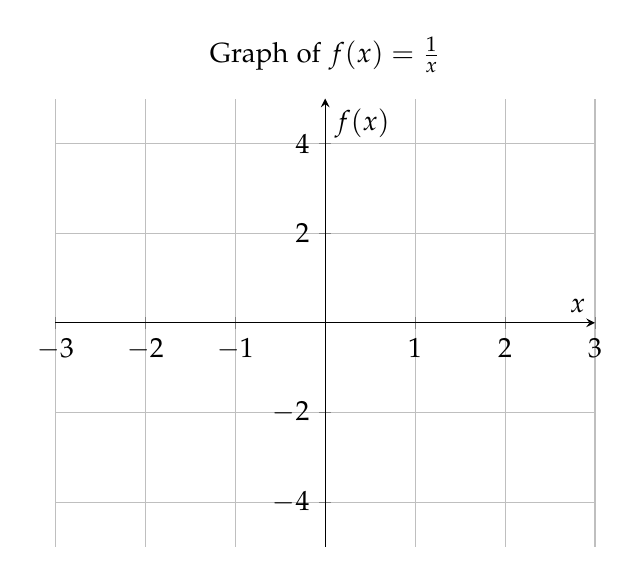
\begin{tikzpicture}
\begin{axis}[
    axis lines = middle,
    xlabel = \( x \),
    ylabel = \( f(x) \),
    grid = both,
    xmin=-3, xmax=3, ymin=-5, ymax=5,
    title = {Graph of \( f(x) = \frac{1}{x} \)}
]
    % \addplot[blue, thick] {1/x};
\end{axis}
\end{tikzpicture}
\end{center}

\subsection*{Graph of \( f(x) = \frac{1}{x^2} \)}

The graph of \( f(x) = \frac{1}{|x|^2} \) has a vertical asymptote at \( x = 0 \) and approaches zero as \( x \to \pm \infty \).

\begin{center}
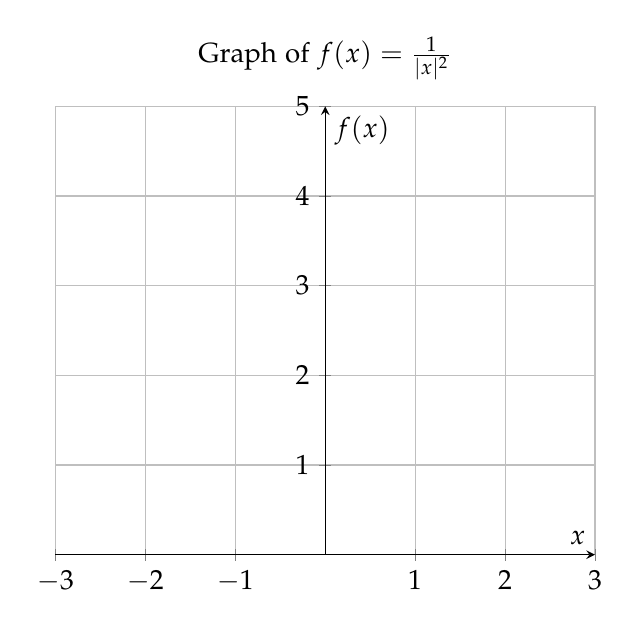
\begin{tikzpicture}
\begin{axis}[
    axis lines = middle,
    xlabel = \( x \),
    ylabel = \( f(x) \),
    grid = both,
    xmin=-3, xmax=3, ymin=0, ymax=5,
    title = {Graph of \( f(x) = \frac{1}{|x|^2} \)}
]
    % \addplot[blue, thick] {1/(x^2)};
\end{axis}
\end{tikzpicture}
\end{center}



%%%

\subsection{Quadratic Functions}

\begin{definition}

% A quadratic function is a polynomial function of degree 2, and it has the general form:

\[
f(x) = ax^2 + bx + c
\]

\end{definition}
The graph of a quadratic function is a parabola, and its shape depends on the coefficient \( a \). If \( a > 0 \), the parabola opens upwards; if \( a < 0 \), it opens downwards. The vertex of the parabola is the point where the graph reaches its minimum or maximum value.

Here we explore different types of quadratic functions, including the basic quadratic function \( f(x) = x^2 \), scaled versions, and transformations.

\subsection*{Graph of \( f(x) = x^2 \)}

The graph of the basic quadratic function \( f(x) = x^2 \) is a parabola with its vertex at the origin \( (0, 0) \). The parabola opens upwards because the coefficient of \( x^2 \) is positive.

\begin{center}
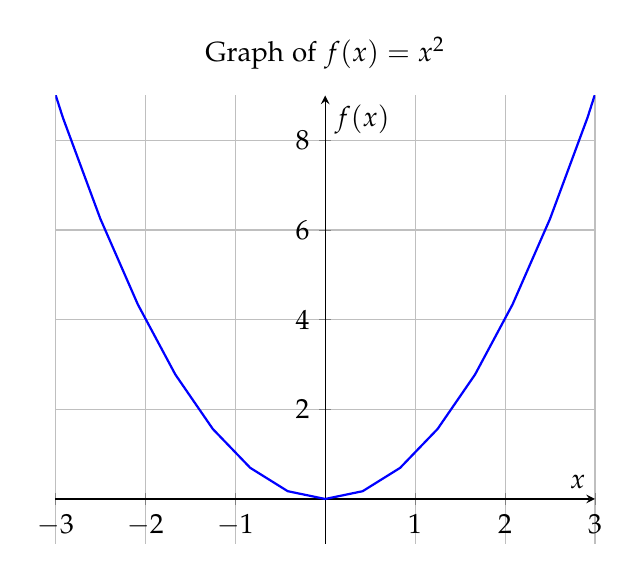
\begin{tikzpicture}
\begin{axis}[
    axis lines = middle, 
    xlabel = \( x \), ylabel = \( f(x) \),
    grid = both, 
    xmin=-3, xmax=3, ymin=-1, ymax=9,
    title = {Graph of \( f(x) = x^2 \)}
]
    \addplot[blue, thick] {x^2};
\end{axis}
\end{tikzpicture}
\end{center}

\subsection*{Graph of \( f(x) = ax^2 \) for Various Values of \( a \)}

In this section, we discuss how the value of \( a \) affects the graph of \( f(x) = ax^2 \). The value of \( a \) controls the "width" and the direction in which the parabola opens.

\subsubsection*{Case 1: \( a = -1 \)}

When \( a = -1 \), the graph of \( f(x) = -x^2 \) is an upside-down parabola with a vertex at \( (0, 0) \).

\begin{center}
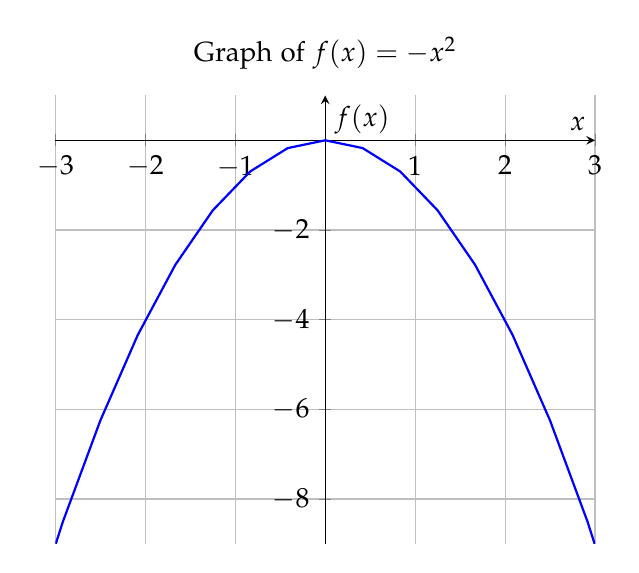
\begin{tikzpicture}
\begin{axis}[
    axis lines = middle, 
    xlabel = \( x \), ylabel = \( f(x) \),
    grid = both, 
    xmin=-3, xmax=3, ymin=-9, ymax=1,
    title = {Graph of \( f(x) = -x^2 \)}
]
    \addplot[blue, thick] {-x^2};
\end{axis}
\end{tikzpicture}
\end{center}

\subsubsection*{Case 2: \( -1 < a < 0 \)}

For \( a \) between -1 and 0, the graph of \( f(x) = ax^2 \) is a vertically compressed parabola that opens downwards. The vertex remains at \( (0, 0) \).

\begin{center}
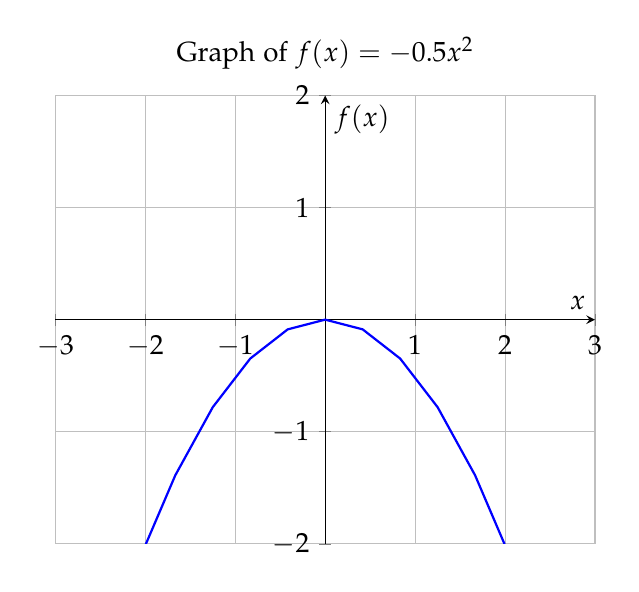
\begin{tikzpicture}
\begin{axis}[
    axis lines = middle, 
    xlabel = \( x \), ylabel = \( f(x) \),
    grid = both, 
    xmin=-3, xmax=3, ymin=-2, ymax=2,
    title = {Graph of \( f(x) = -0.5x^2 \)}
]
    \addplot[blue, thick] {-0.5*x^2};
\end{axis}
\end{tikzpicture}
\end{center}

\subsubsection*{Case 3: \( 0 < a < 1 \)}

For \( a \) between 0 and 1, the graph of \( f(x) = ax^2 \) is a vertically stretched parabola that opens upwards. The vertex remains at \( (0, 0) \).

\begin{center}
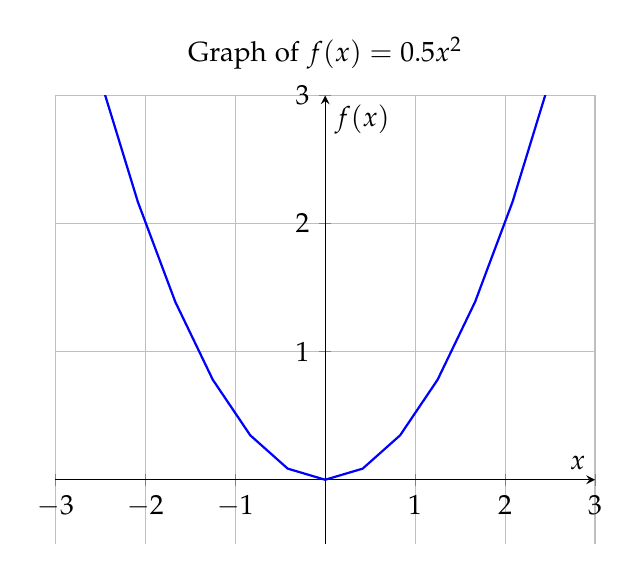
\begin{tikzpicture}
\begin{axis}[
    axis lines = middle, 
    xlabel = \( x \), ylabel = \( f(x) \),
    grid = both, 
    xmin=-3, xmax=3, ymin=-0.5, ymax=3,
    title = {Graph of \( f(x) = 0.5x^2 \)}
]
    \addplot[blue, thick] {0.5*x^2};
\end{axis}
\end{tikzpicture}
\end{center}

\subsubsection*{Case 4: \( a > 1 \)}

When \( a > 1 \), the graph of \( f(x) = ax^2 \) becomes even more vertically stretched, and it opens upwards. The vertex remains at \( (0, 0) \).

\begin{center}
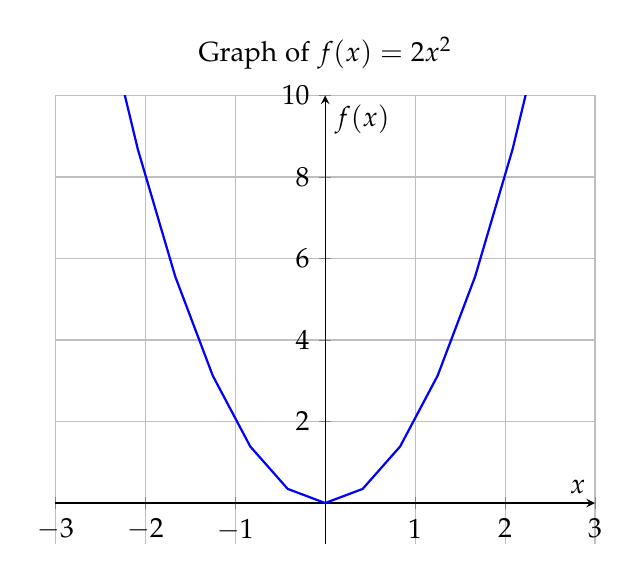
\begin{tikzpicture}
\begin{axis}[
    axis lines = middle, 
    xlabel = \( x \), ylabel = \( f(x) \),
    grid = both, 
    xmin=-3, xmax=3, ymin=-1, ymax=10,
    title = {Graph of \( f(x) = 2x^2 \)}
]
    \addplot[blue, thick] {2*x^2};
\end{axis}
\end{tikzpicture}
\end{center}

\subsection*{Horizontal Transformations of \( f(x) = x^2 \)}

The graph of \( f(x) = x^2 \) can also undergo horizontal transformations. These transformations shift the graph to the left or right.

\subsubsection*{Case 1: \( f(x+2) \)}

The function \( f(x+2) \) shifts the graph of \( f(x) = x^2 \) to the left by 2 units.

\begin{center}
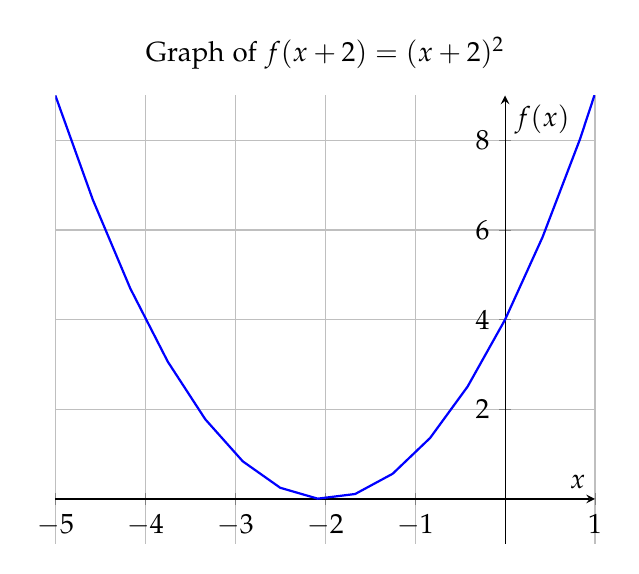
\begin{tikzpicture}
\begin{axis}[
    axis lines = middle, 
    xlabel = \( x \), ylabel = \( f(x) \),
    grid = both, 
    xmin=-5, xmax=1, ymin=-1, ymax=9,
    title = {Graph of \( f(x+2) = (x+2)^2 \)}
]
    \addplot[blue, thick] {(x+2)^2};
\end{axis}
\end{tikzpicture}
\end{center}

\subsubsection*{Case 2: \( f(x-3) \)}

The function \( f(x-3) \) shifts the graph of \( f(x) = x^2 \) to the right by 3 units.

\begin{center}
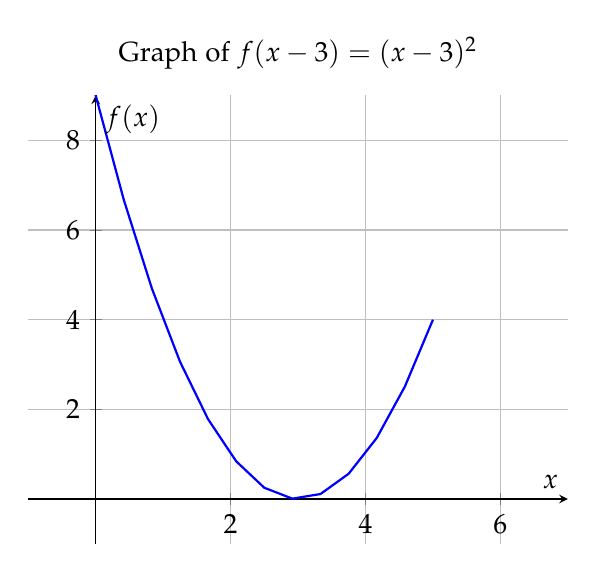
\begin{tikzpicture}
\begin{axis}[
    axis lines = middle, 
    xlabel = \( x \), ylabel = \( f(x) \),
    grid = both, 
    xmin=-1, xmax=7, ymin=-1, ymax=9,
    title = {Graph of \( f(x-3) = (x-3)^2 \)}
]
    \addplot[blue, thick] {(x-3)^2};
\end{axis}
\end{tikzpicture}
\end{center}

\subsection*{Vertical Transformations of \( f(x) = x^2 \)}

In addition to horizontal transformations, vertical transformations can shift the graph of \( f(x) = x^2 \) up or down.

\subsubsection*{Case 1: \( f(x) = x^2 + 3 \)}

The function \( f(x) = x^2 + 3 \) shifts the graph of \( f(x) = x^2 \) upwards by 3 units.

\begin{center}
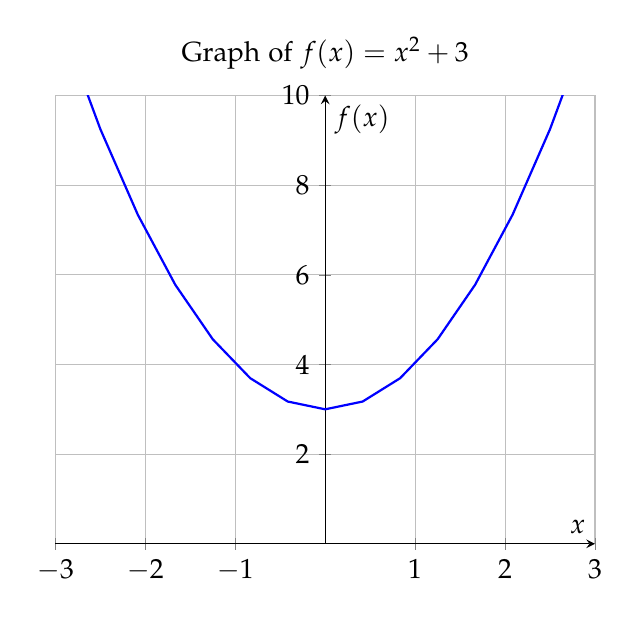
\begin{tikzpicture}
\begin{axis}[
    axis lines = middle, 
    xlabel = \( x \), ylabel = \( f(x) \),
    grid = both, 
    xmin=-3, xmax=3, ymin=0, ymax=10,
    title = {Graph of \( f(x) = x^2 + 3 \)}
]
    \addplot[blue, thick] {x^2 + 3};
\end{axis}
\end{tikzpicture}
\end{center}

\subsubsection*{Case 2: \( f(x) = x^2 - 1 \)}

The function \( f(x) = x^2 - 1 \) shifts the graph of \( f(x) = x^2 \) downwards by 1 unit.

\begin{center}
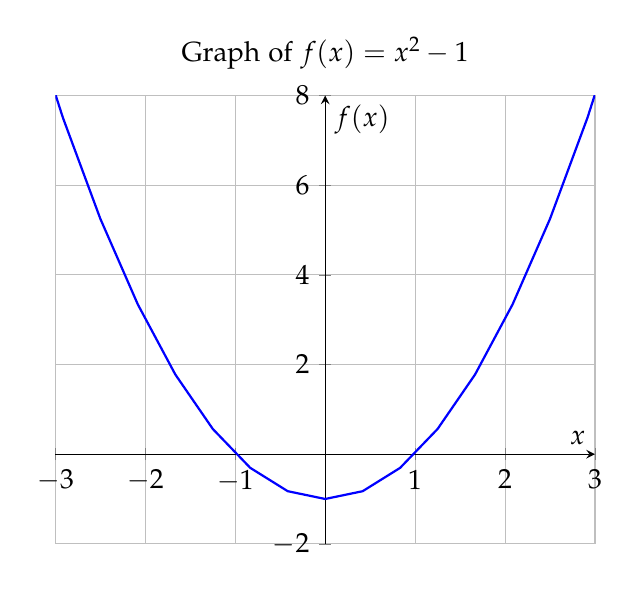
\begin{tikzpicture}
\begin{axis}[
    axis lines = middle, 
    xlabel = \( x \), ylabel = \( f(x) \),
    grid = both, 
    xmin=-3, xmax=3, ymin=-2, ymax=8,
    title = {Graph of \( f(x) = x^2 - 1 \)}
]
    \addplot[blue, thick] {x^2 - 1};
\end{axis}
\end{tikzpicture}
\end{center}

\subsubsection*{Case 3: \( f(x) = (x-2)^2 + 3 \)}

The function \( f(x) = (x-2)^2 + 3 \) shifts the graph of \( f(x) = x^2 \) to the right by 2 units and upwards by 3 units.

\begin{center}
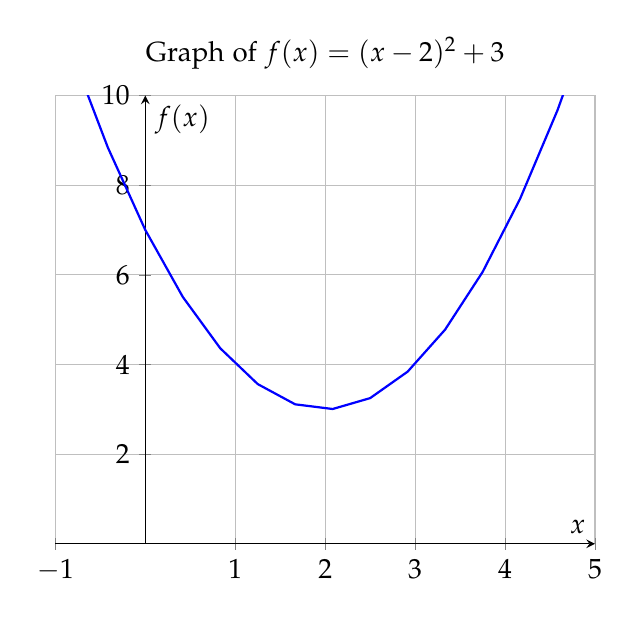
\begin{tikzpicture}
\begin{axis}[
    axis lines = middle, 
    xlabel = \( x \), ylabel = \( f(x) \),
    grid = both, 
    xmin=-1, xmax=5, ymin=0, ymax=10,
    title = {Graph of \( f(x) = (x-2)^2 + 3 \)}
]
    \addplot[blue, thick] {(x-2)^2 + 3};
\end{axis}
\end{tikzpicture}
\end{center}
g

\subsection{Quotient of Two Functions}

Given two functions \( f(x) \) and \( g(x) \), their quotient is defined as:

\[
\frac{f(x)}{g(x)} = \frac{x^2 - 2}{x + 2}
\]

In this case, we have:
\[
f(x) = x^2 - 2 \quad \text{and} \quad g(x) = x + 2
\]

The domain of the quotient function \( \frac{f(x)}{g(x)} \) is determined by the domain of both \( f(x) \) and \( g(x) \), with the restriction that \( g(x) \neq 0 \), since division by zero is undefined. Therefore, we must exclude values of \( x \) where \( g(x) = 0 \). Solving \( g(x) = x + 2 = 0 \) gives \( x = -2 \). Hence, the domain of \( \frac{f(x)}{g(x)} \) is all real numbers except \( x = -2 \).

\subsection*{Finding the Quotient Function \( \frac{f(x)}{g(x)} \)}

We now compute the quotient function \( \frac{f(x)}{g(x)} \):

\[
\frac{f(x)}{g(x)} = \frac{x^2 - 2}{x + 2}
\]

This is the simplified form of the quotient. It is important to note that this function is undefined at \( x = -2 \), as discussed earlier.

\subsection*{Evaluating \( \frac{f(x)}{g(x)} \) at \( x = 2 \)}

To evaluate \( \frac{f}{g}(2) \), we substitute \( x = 2 \) into the quotient function:

\[
\frac{f}{g}(2) = \frac{f(2)}{g(2)} = \frac{2^2 - 2}{2 + 2} = \frac{4 - 2}{4} = \frac{2}{4} = \frac{1}{2}
\]

Thus, \( \frac{f}{g}(2) = \frac{1}{2} \).

\subsection*{Evaluating \( \frac{f(x)}{g(x)} \) at \( x = t \)}

To evaluate \( \frac{f}{g}(t) \), we substitute \( x = t \) into the quotient function:

\[
\frac{f}{g}(t) = \frac{f(t)}{g(t)} = \frac{t^2 - 2}{t + 2}
\]

Thus, the value of the quotient function at \( x = t \) is:

\[
\frac{f}{g}(t) = \frac{t^2 - 2}{t + 2}
\]


The quotient of two functions \( f(x) = x^2 - 2 \) and \( g(x) = x + 2 \) is given by:

\[
\frac{f(x)}{g(x)} = \frac{x^2 - 2}{x + 2}
\]

We computed:
\[
\frac{f}{g}(2) = \frac{1}{2}
\]
and the general form for \( \frac{f}{g}(t) \) is:

\[
\frac{f}{g}(t) = \frac{t^2 - 2}{t + 2}
\]

The domain of this function is all real numbers except \( x = -2 \), where the function is undefined due to division by zero.



\subsection{Applications}

In business economics, functions can be used to underst the relationship between costs, revenues, and profits. 
% \subsection{Fixed Costs}

% Fixed costs are the costs that do not change with the level of output produced by a company. Common examples of fixed costs include rent, salaries of permanent employees, and insurance premiums. 

% \subsection{Marginal Costs}

% Marginal cost refers to the additional cost incurred by producing one more unit of output.
 % It is a key concept in microeconomics that helps businesses determine the cost efficiency of increasing production. The marginal cost is the derivative of the total cost function with respect to the quantity produced.

% Mathematically, marginal cost is expressed as:

% \[
% MC(x) = \frac{dC(x)}{dx}
% \]

% where \( C(x) \) is the total cost function, and \( x \) is the quantity of output produced.

% The marginal cost helps a company decide whether increasing production is profitable. If the marginal cost is greater than the price at which the product is sold, it might not be profitable to increase production.

\begin{definition}
[Cost Function]

The cost function, denoted as \( C(x) \), represents the total cost incurred by a company to produce \( x \) units of output. 

\[
C(x) = C_{\text{fixed}} + C_{\text{variable}}(x)
\]

where:
\begin{itemize}
\item \( C_{\text{fixed}} \) is the fixed cost (constant),
\item \( C_{\text{variable}}(x) \) is the variable cost, which typically depends on the number of units produced, \( x \).
\end{itemize}

\end{definition}

For example, a simple cost function might look like:

\[
C(x) = 500 + 10x
\]

where 500 is the fixed cost, and \( 10x \) represents the variable cost per unit produced.

\begin{definition}
[Revenue Function]

The revenue function, denoted as \( R(x) \), represents the total revenue generated by selling \( x \) units of output at a price \( p(x) \) per unit. The revenue function is given by the product of the price per unit and the quantity of output sold.

\[
R(x) = p(x) \cdot x
\]

where:
\begin{itemize}
\item \( p(x) \) is the price per unit, which can be constant or variable depending on the market conditions,
\item \( x \) is the number of units sold.
\end{itemize}

\end{definition}

For example, if the price per unit is constant at \( p = 20 \), the revenue function would be:

\[
R(x) = 20x
\]

This means that for every unit sold, the company generates 20 units of revenue.

\begin{definition}
[Profit Function]


The profit function, denoted as \( P(x) \), represents the difference between total revenue and total cost. It shows how much money a company makes (or loses) from producing and selling \( x \) units of output.

\[
P(x) = R(x) - C(x)
\]

where:
\begin{itemize}
\item \( R(x) \) is the revenue function,
\item \( C(x) \) is the cost function.
\end{itemize}
\end{definition}

For example, if the revenue function is \( R(x) = 20x \) and the cost function is \( C(x) = 500 + 10x \), the profit function would be:

\[
P(x) = (20x) - (500 + 10x) = 10x - 500
\]

This profit function shows that the company makes a profit of \( 10x - 500 \) when producing and selling \( x \) units. The company will break even when \( P(x) = 0 \), which occurs when:

\[
10x - 500 = 0 \quad \Rightarrow \quad x = 50
\]

Thus, the company needs to sell at least 50 units to cover its costs and start making a profit.

\subsubsection*{Example }
Write a linear cost function for the following situations. 
A ski resort charges a snowboard rental fee of 30 dollars
plus 5 dollars per hour.
\textbf{Solution}

A linear cost function is typically written in the form:
\[
C(x) = mx + b
\]
where:
- \( C(x) \) is the total cost,
- \( m \) is the variable cost per unit of \( x \),
- \( b \) is the fixed cost,
- \( x \) is the number of hours.

Therefore 

\[
C(x) = 5x + 30
\]

\subsubsection*{Example }
Write a linear cost function for the following situations.
A parking garage charges 7 dollars plus 50 cents per half$-$hour.



\textbf{Solution}

\[
C(x) = 0.50x + 7
\]




\newpage


\section{Polyonomial Functions}
\begin{definition} [Polynomial Functions]
  A polynomial function of degree $n$ is defined as 
  \[
  f(x) = a_n x^n + a_{n-1} x^{n-1} + \cdots + a_1 x + a_0
  \]
  
  where $a_{n } \neq 0$
\end{definition}

\subsection*{Remarks}
\begin{itemize}
\item The degree \( n \) is the highest exponent of \( x \) in the polynomial.
\item \( a_n \) is the leading coefficient. 
\item A linear functions is a Polynomial function of degree 1.
\item A quadratic functions is a Polynomial function of degree 2.
\item A cubic functions is a Polynomial function of degree 3.
\end{itemize}


\subsection{Zeros/Roots of a Polynomial}

TBD!
\subsection{Relative Maximum and Minimum Values of a Polynomial}
TBD!

\subsection{Graphing Polynomial Functions}

The behavior of the graph of a polynomial is significantly influenced by both the degree of the polynomial and the sign and magnitude of the leading coefficient. 



\subsubsection{Impact of the Leading Coefficient on the Graph}

The leading coefficient, \( a_n \), plays a crucial role in determining the end behavior of the polynomial graph as \( x \to \infty \) or \( x \to -\infty \). Specifically, it influences the direction in which the graph will tend as \( x \) moves away from the origin.

\subsection*{Case 1: \( a_n > 0 \) and \(n\) is Even}

When the leading coefficient \( a_n \) is positive and the degree \( n \) of the polynomial is even, the graph of the polynomial exhibits the following behavior:


\begin{itemize}
    \item As \( x \to \pm \infty \), the graph tends to \( +\infty \).
\end{itemize}

Thus, in this case, both ends of the graph will rise to \( +\infty \). 

\begin{example}
  Consider   \( f(x) = x^4 - 3x^3 + x \).
  \begin{itemize}
  \item Degree = 4.
  \item Leadign Coeffecient = 1 $>$ 0.
  \end{itemize}

\begin{figure}[H]
  \centering
  \includegraphics[scale=0.2]{"./fig/case_1.png"}
\end{figure}
\end{example}


\subsection*{Case 2: \( a_n > 0 \) and \(n\) is Odd}


When the leading coefficient \( a_n \) is positive and the degree \( n \) of the polynomial is odd, the graph of the polynomial exhibits the following behavior:

\begin{itemize}
    \item As \( x \to \pm \infty \), the graph tends to \( \pm \infty \).
\end{itemize}


\begin{example}
\(f(x) = x^{5}+3x^{2}-3x\ -1\)
  \begin{itemize}
  \item Degree = 5.
  \item Leadign Coeffecient = 1 $>$ 0.
  \end{itemize}

\begin{figure}[H]
  \centering
  \includegraphics[scale=0.2]{"./fig/case_3.png"}
\end{figure}
\end{example}

\subsection*{Case 3: \( a_n < 0 \) and \(n\) is Even}


When the leading coefficient \( a_n \) is negative and the degree \( n \) of the polynomial is even, the graph of the polynomial exhibits the following behavior:

\begin{itemize}
    \item As \( x \to \pm \infty \), the graph tends to \( - \infty \).
\end{itemize}


\begin{example}
Consider \( f(x) =-1.2x^{4}-3x^{3}+x\)
  Consider   \( f(x) = -2x^6 - 2x^3 + 2 \).
  \begin{itemize}
  \item Degree = 4.
  \item Leadign Coeffecient = -1.2 $<$ 0.
  \end{itemize}


\begin{figure}[H]
  \centering
  \includegraphics[scale=0.2]{"./fig/case_2.png"}
\end{figure}
\end{example}

\subsection*{Case 4: \( a_n < 0 \) and \(n\) is Odd}

When the leading coefficient \( a_n \) is negative and the degree \( n \) of the polynomial is odd, the graph of the polynomial exhibits the following behavior:

\begin{itemize}
    \item As \( x \to \pm \infty \), the graph tends to \( \mp \infty \).
\end{itemize}


\begin{example}
  Consider   \( f(x) =-3x^{3}+3x^{2\ \ }-2
 \).
  \begin{itemize}
  \item Degree = 6.
  \item Leadign Coeffecient = -1 $<$ 0.
  \end{itemize}

\begin{figure}[H]
  \centering
  \includegraphics[scale=0.2]{"./fig/case_4.png"}
\end{figure}
\end{example}




- Graph of cubic equations
- Graph of quartic equations
- Find the degree and leading coefficient of a polynomial by looking at its graph
- Horizontal and vertical asymptotes
\section{Rational Functions}
\begin{definition}[Rational Functions]
A rational function is a function that can be expressed as the ratio of two polynomials, i.e.,
\[
f(x) = \frac{P(x)}{Q(x)}
\]
where \( P(x) \) and \( Q(x) \) are polynomials and \( Q(x) \neq 0 \). 
\end{definition}
The behavior of a rational function is often analyzed using asymptotes, which are lines that the graph of the function approaches but never touches.

There are two main types of asymptotes: vertical asymptotes and horizontal asymptotes.


\subsection*{Vertical Asymptotes}

A vertical asymptote occurs when the function approaches infinity or negative infinity as \( x \) approaches a certain value from the left or right.

These asymptotes are generally found by determining where the denominator of the rational function equals zero, provided that the numerator does not also equal zero at the same value.

Steps to Find Vertical Asymptotes:
\begin{itemize}
\item Set the denominator \( Q(x) = 0 \) and solve for \( x \).
\item If the numerator \( P(x) \) does not equal zero at the same values of \( x \), then those values are vertical asymptotes.
\end{itemize}

\begin{example}
Find the Vertical Asymptotes of \( f(x) = \frac{1}{x^2 - 4} \)

\begin{figure}[H]
  \centering
  \includegraphics[scale=0.2]{"./fig/vert_asym.png"}
\end{figure}
\end{example}

Consider the rational function

\[
f(x) = \frac{1}{x^2 - 4}
\]

To find the vertical asymptotes, we set the denominator equal to zero:

\[
x^2 - 4 = 0.
\]

Solving this equation, we get

\[
x^2 = 4 \quad \Rightarrow \quad x = \pm 2.
\]

Since the numerator is not zero at \( x = 2 \) or \( x = -2 \), the vertical asymptotes of this function are at

\[
x = 2 \quad \text{and} \quad x = -2
\]

Thus, the graph of \( f(x) \) has vertical asymptotes at \( x = 2 \) and \( x = -2 \).

\subsection*{Horizontal Asymptotes}

A horizontal asymptote describes the behavior of a rational function as \( x \to \infty \) or \( x \to -\infty \).

The horizontal asymptote indicates the value that the function approaches as \( x \) becomes very large or very small.

Steps to Find Horizontal Asymptotes:

\begin{itemize}
    \item If \( \deg(P(x)) < \deg(Q(x)) \), then the horizontal asymptote is \( y = 0 \).
    \item If \( \deg(P(x)) = \deg(Q(x)) \), then the horizontal asymptote is \( y = \frac{\text{leading coefficient of } P(x)}{\text{leading coefficient of } Q(x)} \).
    \item If \( \deg(P(x)) > \deg(Q(x)) \), there is no horizontal asymptote (but there might be an oblique/slant asymptote).
\end{itemize}

\begin{example}
Find the Horizontal Asymptote of \( f(x) = \frac{3x^2 + 5}{2x^2 + 7} \)
\end{example}

\textbf{Solution}

Here, both the numerator and the denominator are of degree 2. Therefore, we apply the second rule:

\[
y = \frac{\text{leading coefficient of } P(x)}{\text{leading coefficient of } Q(x)} = \frac{3}{2}
\]

Thus, the horizontal asymptote of the function is:

\[
y = \frac{3}{2}
\]


\begin{figure}[H]
  \centering
  \includegraphics[scale=0.2]{"./fig/ho_asym1.png"}
\end{figure}

\begin{example}
Find the Horizontal Asymptote of \( f\left(x\right)\ =\ \frac{3x-2}{2x^{2}+7}\)



\begin{figure}[H]
  \centering
  \includegraphics[scale=0.2]{"./fig/ho_asym2.png"}
\end{figure}

\end{example}
\begin{example}
Find the Horizontal Asymptote of \( f(x) = \frac{x^3 - 4x}{x^2 + 1} \)
\end{example}

\textbf{Solution:}

Here, the degree of the numerator is 3 and the degree of the denominator is 2. Since \( \deg(P(x)) > \deg(Q(x)) \), there is no horizontal asymptote. Instead, there may be an oblique or slant asymptote.

\begin{figure}[H]
  \centering
  \includegraphics[scale=0.2]{"./fig/ho_asym3.png"}
\end{figure}
\section{Exponential Functions}

\begin{definition}
[Exponential Function]
An exponential function is generally given by:
\[
f(x) = a^x
\]
where \( a \neq 1 \) \( a>0 \). 
\end{definition}

The overall behavior of plot of $f(x)$ depends whether $0<a<1$ or $a>1$.

\subsection*{Graph of \(a^{x}\) when \(a<0\)}
\begin{figure}[H]
  \centering
  \includegraphics[scale=0.15]{"./fig/exp_1.png"}
\end{figure}
\subsection*{Graph of \(a^{x}\) when \(0<a<1\)}

\begin{figure}[H]
  \centering
  \includegraphics[scale=0.15]{"./fig/exp_2.png"}
\end{figure}

\begin{example}
  Plot the graph of \( f\left(x\right)\ =\ 6-5^{-x}\).
\begin{itemize}
\item Step 1. Plot \( 5^{-x} \) or $ \left( \frac{1}{5} \right)^{x} (black)$
\item Step 2.  Reflect  \( 5^{-x} \) to obtain \( -5^{-x} \) (blue)
\item Step 3.  Vertically translate  \( -5^{-x} \) to obtain \( 6-5^{-x} \) (green)
\end{itemize}

\begin{figure}[H]
  \centering
  \includegraphics[scale=0.15]{"./fig/exp_tr.png"}
\end{figure}
\end{example}


\subsection{Solving Exponential Equations}

\begin{example} 

  Solve \(7^{x} = 343 \) for $x$

  Since \(7^{x} = 7^{3} \), therefor $x=3$


\end{example}


\begin{example}
  Solve \(64^{3x-1} = 16^{2x+3}\) for \(x\).
  
  Since \(64 = 2^6\) and \(16 = 2^4\), therefore
  
  \[
  \left( 2^6 \right)^{3x-1} = \left( 2^4 \right)^{2x+3}
  \]
  \[
  2^{6(3x-1)} = 2^{4(2x+3)}
  \]
  
 and
  
  \(6(3x-1) = 4(2x+3) \)
  or
  \(18x - 6 = 8x + 12 \)
  
  which results in 
  \(18x - 8x = 12 + 6 \)

   and gives us 
   \(x = \frac{18}{10} = \frac{9}{5} \)
  


\end{example}

\section{Logarithmic Functions}

We can express logarithmic equations in exponential form as follows:

\[
2^4 = 16 \quad \text{is equivalent to} \quad 4 = \log_2 16
\]
\[
3^2 = 9 \quad \text{is equivalent to} \quad 2 = \log_3 9
\]
\[
5^6 = 625 \quad \text{is equivalent to} \quad 6 = \log_5 625
\]
\[
10^x = 1000 \quad \text{is equivalent to} \quad ?
\]
\[
10^x = 15 \quad \text{is equivalent to} \quad ?
\]
\begin{definition}
[Logarithm]
A logarithm is the inverse operation of exponentiation. If we have an equation of the form:

\[
a^x = b
\]

then the logarithm of \( b \) with base \( a \) is defined as:

\[
\log_a b = x
\]
\end{definition}
This means that the logarithm of \( b \) with base \( a \) is the exponent \( x \) to which \( a \) must be raised to obtain \( b \).


\begin{itemize}
    \item The base \( a \) of a logarithm is a positive real number (except 1), and it determines the base of the exponential function.
    \item The argument \( b \) is the value for which we are finding the logarithm.
    \item The logarithm \( \log_a b \) gives the exponent to which the base \( a \) must be raised to equal \( b \).
\end{itemize}

\begin{example}
Solving a Basic Logarithmic Equation:

\[
\log_2 8 = x
\]

This asks: "To what power must 2 be raised to give 8?" We know that:

\[
2^3 = 8
\]

Thus:

\[
\log_2 8 = 3
\]

\end{example}

\begin{example}
 Converting Between Exponential and Logarithmic Form

The equation \( 10^x = 1000 \) can be written in logarithmic form as:

\[
\log_{10} 1000 = x
\]

Since \( 10^3 = 1000 \), we find that:

\[
\log_{10} 1000 = 3
\]

\end{example}


\begin{example}
Solving for \( x \) in a Logarithmic Equation
\end{example}

Solve the equation:

\[
\log_5 x = 3
\]

This means that \( 5^3 = x \), and solving for \( x \):

\[
x = 5^3 = 125
\]

Thus, the solution is \( x = 125 \).

\subsection{Properties of Logarithms}

Logarithms have several important properties that can help simplify calculations:

\begin{itemize}
 \item
\[
 \log_{a}1 = 0
\]

 \item
\[
 \log_{a}a = 1
\]
\item \textbf{Product Rule}
\[
\log_a (xy) = \log_a x + \log_a y
\]
\item \textbf{Quotient Rule}
\[
\log_a \left( \frac{x}{y} \right) = \log_a x - \log_a y
\]
\item \textbf{Power Rule}
\[
\log_a (x^n) = n \log_a x
\]
\item \textbf{Change of Base Formula}
\[
\log_a b = \frac{\log_c b}{\log_c a}
\]
\end{itemize}

\begin{example}
Change of Base Formula:
Using the change of base formula, we can compute \( \log_2 8 \) using base 10 logarithms:

\[
\log_2 8 = \frac{\log_{10} 8}{\log_{10} 2}
\]

\end{example}

\subsection{Common Logarithms and Natural Logarithms}

There are two special types of logarithms that are commonly used:

\subsection*{Common Logarithm}

The common logarithm has base 10 and is usually written as \( \log x \) (without specifying the base):

\[
\log x = \log_{10} x
\]

\subsection*{Natural Logarithm}

The natural logarithm has base \( e \) (where \( e \approx 2.718 \)) and is usually written as \( \ln x \):

\[
\ln x = \log_e x
\]

For example:

\[
\ln e = 1
\]

% \begin{example}
%   Use the properties of logarithms to write the expression as a sum,
%   difference, or product of simpler logarithms.
%   \begin{itemize}
%   \item $\log_{4}\sqrt{5x}$
%   \item $\log_{2} \left(\frac{4x}{5y} \right)$
%   \item $\log_{4}\sqrt{5x}$
%   \item $\ln\left (\frac{\sqrt{5x}}{\sqrt[3]{4}} \right)$ %cube root in last part
%   % \item $\log_{4}\sqrt{5x}$
%   \end{itemize}
% \end{example}

% \begin{example}
%   Solve the equation for $x$.
%   \begin{itemize}
%   \item $\log_{x} 625 = 4$ 
%   \item $\log_{4} (x+1) - \log_{4}(x-1)  = 1$ 
%   \item $\ln x + \ln 3x = 5 $
%   \item $e^{x+1} = 18$ 
%   \end{itemize}
% \end{example}

% \subsection{Applicatons}
% - Applications, Word Problems

%%% Local Variables:
%%% mode: LaTeX
%%% TeX-master: t
%%% End:

\begin{example}
  Use the properties of logarithms to write the expression as a sum,
  difference, or product of simpler logarithms.
  \begin{enumerate}
  \item $\log_{4}\sqrt{5x}$
  \item $\log_{2} \left(\frac{4x}{5y} \right)$
  \item $\log_{4}\sqrt{5x}$
  \item $\ln\left (\frac{\sqrt{5x}}{\sqrt[3]{4}} \right)$ %cube root in last part
  % \item $\log_{4}\sqrt{5x}$
  \end{enumerate}
\end{example}

\textbf{Solution:}
\begin{enumerate}
\item Using power rule we get
  \[
  \log_4 \sqrt{5x} = \log_4 (5x)^{1/2} = \frac{1}{2} \log_4 (5x)
  \]
  Since
  \[
   \log_4 (5x) =   \log_4 5 + \log_4 x 
  \]
  therefore
  \[
  \log_4 \sqrt{5x} = \frac{1}{2} \log_4 5 + \frac{1}{2} \log_4 x
\]

\item 
  \[
  \log_2 \left( \frac{4x}{5y} \right) = \log_2 (4x) - \log_2 (5y)
  \]
  since,
  \[
  \log_2 (4x) = \log_2 4 + \log_2 x
  \]
  and 
  \[
  \log_2 (5y) = \log_2 5 + \log_2 y
  \]
  therefore:
  \[
  \log_2 \left( \frac{4x}{5y} \right)=\log_2 4 + \log_2 x - (\log_2 5 + \log_2 y)
  \]
  Since \(\log_2 4 = \log_2 2^{2} = 2 \log_2 2 = 2\), the final expression is:
  \[
  \log_2 \left( \frac{4x}{5y} \right)=2 - \log_2 5 + \log_2 x - \log_2 y
  \]
\item Try yourself!
\item Try yourself!
\end{enumerate}



\begin{example}
  Solve the equation for $x$.
  \begin{enumerate}
  \item $\log_{x} 625 = 4$ 
  \item $\log_{4} (x+1) - \log_{4}(x-1)  = 1$ 
  \item $\ln x + \ln 3x = 5 $
  \item $e^{x+1} = 18$ 
  \end{enumerate}
\end{example}

\subsection{Applicatons}

\begin{example}
The census bureau for a large country has reported that the country is becoming more diverse. The projected population (in millions) of a certain minority is modeled by the exponential function
\[
h(t) = 37.67 \times (1.023)^t \quad \text{where} \quad 0 \leq t \leq 50.
\]
for the years 2000 to 2050.
Estimate in what year the minority's population will double the 2005 population of 42.21 million. 

\end{example}

\textbf{Solution}
We are given the population model:
\[
h(t) = 37.67 \times (1.023)^t
\]
and the population in 2005 is 42.21 million, we can verify this by.
\[
h(5) = 37.67 \times (1.023)^{5} \approx 42.21
\]
We need to find the year when the population doubles 
\(
2 \times 42.21 = 84.42 \text{ million}.
\)
Therefore
\[
84.42 = 37.67 \times (1.023)^t.
\]
and  Solve for \( t \)
\[
\frac{84.42}{37.67} = (1.023)^t,
\]
\[
2.24 = (1.023)^t.
\]

Take the natural logarithm (or any logarithm) of both sides, we get
\[
\ln(2.24) = t \ln(1.023).
\]

therefore:
\[
t = \frac{\ln(2.24)}{\ln(1.023)} \approx 
 0.8047, \quad \ln(1.023) \approx 0.0227,
\]
we get:
\[
t \approx \frac{0.8047}{0.0227} \approx 35.44.
\]

Thus, the population will double in approximately the year 2035.

\begin{example}
Find the present value of a deposit of \$40,000 at an interest rate of 4.1\% compounded continuously for 10 years.
\end{example}

\textbf{Solution}
The formula for the present value \( P \) when the amount \( A \) is compounded continuously is given by:
\[
A = P e^{rt}
\]
where \( r \) is the interest rate (4.1\% or 0.041).

We are given \( A = 40,000 \), \( r = 0.041 \), and  \( t = 10 \). 

\[
40,000 = P e^{0.041 \times 10}
\]
\[
40,000 = P e^{0.41}
\]

\[
P = \frac{40,000}{e^{0.41}}.
\]

\[
P \approx \frac{40,000}{1.506} \approx 26,546.01.
\]

% \input{week3.tex}

\newpage
\section{Limits}


\begin{example}
  \label{ex:num_lim}
  What value $f(x) = x^{2}$ approaches to, when x approaches to 2.

  In mathematical notation $f(x) \to ?$ when $x \to 2$
\end{example}

\textbf{Left-Hand Limit Table for \( f(x) = x^2 \) as \( x \to 2^{-} \)}

\begin{longtable}{|c|c|}
\hline
\textbf{x} & \textbf{f(x) = \( x^2 \)} \\
\hline
\endfirsthead
\hline
\textbf{x} & \textbf{f(x) = \( x^2 \)} \\
\hline
\endhead
1.9 & 3.61 \\
\hline
1.99 & 3.9601 \\
\hline
1.999 & 3.996001 \\
\hline
1.9999 & 3.99960001 \\
\hline
1.99999 & 3.9999600001 \\
\hline
\end{longtable}

\textcolor{red}{We say that $f(x) \to 4 $ as $x \to 2^{-}$}

Or

\textcolor{red}{Equivalently $ lim_{x \to 2^{-}}f(x) = 4$}  

\textbf{Right-Hand Limit Table for \( f(x) = x^2 \) as \( x \to 2^{+} \)}

\begin{longtable}{|c|c|}
\hline
\textbf{x} & \textbf{f(x) = \( x^2 \)} \\
\hline
\endfirsthead
\hline
\textbf{x} & \textbf{f(x) = \( x^2 \)} \\
\hline
\endhead
2.1 & 4.41 \\
\hline
2.01 & 4.0401 \\
\hline
2.001 & 4.004001 \\
\hline
2.0001 & 4.00040001 \\
\hline
2.00001 & 4.0000400001 \\
\hline
\end{longtable}

\textcolor{red}{We say that $f(x) \to 4 $ as $x \to 2^{+}$}

Or

\textcolor{red}{Equivalently $ lim_{x \to 2^{+}}f(x) = 4$}  


\textcolor{cyan}{ $ lim_{x \to 2^{+}}f(x) = lim_{x \to 2^{-}}f(x) = 4$}  

\textcolor{cyan}{ we conclude that $ lim_{x \to 2}f(x) =  4$}  

We say that limit of $f(x)=x^{2}$ is 4 when $x$ approaches to 2.


\begin{figure}[H]
  \centering
  \includegraphics[scale=0.5]{"./fig/num_lim_exm_1.png"}
  \caption{\label{fig:fig_label} Figure corresponding to example \eqref{ex:num_lim} Taken form the textbook, page 135. }
\end{figure}


\begin{example}
  \label{ex:num_lim2}
What value  $f(x) = \frac{x^3 - 2x^2}{x - 2} $ approaches to, when x approaches to 2.

\end{example}
\textbf{Left-hand Limit Table for \( f(x) = \frac{x^3 - 2x^2}{x - 2} \) as \( x \to 2 \)}

\begin{longtable}{|c|c|}
\hline
\textbf{x} & \textbf{f(x) = \( \frac{x^3 - 2x^2}{x - 2} \)} \\
\hline
\endfirsthead
\hline
\textbf{x} & \textbf{f(x)} \\
\hline
\endhead
1.9 & 3.61 \\
\hline
1.99 & 3.9601 \\
\hline
1.999 & 3.996001 \\
\hline
1.9999 & 3.99960001 \\
\hline
1.99999 & 3.9999600001 \\
\hline
\end{longtable}

\textcolor{red}{We say that $f(x) \to 4 $ as $x \to 2^{-}$}

Or

\textcolor{red}{Equivalently $ lim_{x \to 2^{-}}f(x) = 4$}  
\textbf{Right-hand Limit Table for \( f(x) = \frac{x^3 - 2x^2}{x - 2} \) as \( x \to 2 \)}

\begin{longtable}{|c|c|}
\hline
\textbf{x} & \textbf{f(x) = \( \frac{x^3 - 2x^2}{x - 2} \)} \\
\hline
\endfirsthead
\hline
\textbf{x} & \textbf{f(x)} \\
\hline
\endhead
2.1 & 4.41 \\
\hline
2.01 & 4.0401 \\
\hline
2.001 & 4.004001 \\
\hline
2.0001 & 4.00040001 \\
\hline
2.00001 & 4.0000400001 \\
\hline
\end{longtable}

\textcolor{red}{We say that $f(x) \to 4 $ as $x \to 2^{+}$}

Or

\textcolor{red}{Equivalently $ lim_{x \to 2^{+}}f(x) = 4$}  

\textcolor{cyan}{ $ lim_{x \to 2^{+}}f(x) = lim_{x \to 2^{-}}f(x) = 4$}  

\textcolor{cyan}{ we conclude that $ lim_{x \to 2}f(x) =  4$}  

We say that limit of $f(x)=x^{2}$ is 4 when $x$ approaches to 2.


\begin{figure}[H]
  \centering
  \includegraphics[scale=0.5]{"./fig/num_lim_exm_2.png"}
  \caption{\label{fig:fig_label2} Figure corresponding to example \eqref{ex:num_lim2} Taken form the textbook, page 136. }
\end{figure}

\begin{example}
  Find algebraically the limit of  $f(x) = \frac{x^3 - 2x^2}{x - 2} $ when $x \to  2$

  

\end{example}

\textbf{Solution}



We can simplify the expression for \( f(x) \),
by factoring the numerator:
\[
f(x) = \frac{x^2(x - 2)}{x - 2}
\]
For \( x \neq 2 \), the expression simplifies to:


\[
f(x) = \frac{x^2 \cancel{(x - 2)}}{ \cancel{x - 2}}
\]

\[
f(x) = x^2
\]
which is the same now as example \eqref{ex:num_lim}

Therefore, we conclude that
\[
\lim_{x \to 2} f(x) = 2^2 = 4
\]



No we are ready to define limite formally.

\begin{definition}[Left-Hand Limit]
The left-hand limit of \( f(x) \) as \( x \to a \) is defined as:
\[
\lim_{x \to a^-} f(x) = L
\]
which means that as \( x \) approaches \( a \) from the left, the function \( f(x) \) approaches \( L \).

\end{definition}

\begin{definition}[Right-Hand Limit]

The right-hand limit of \( f(x) \) as \( x \to a \) is defined as:
\[
\lim_{x \to a^+} f(x) = L
\]
which means that as \( x \) approaches \( a \) from the right, the function \( f(x) \) approaches \( L \).

\end{definition}



\begin{definition}[Limit]

The limit of \( f(x) \) as \( x \to a \) is defined as:
\[
\lim_{x \to a} f(x) = L
\]
which means that as \( x \) approaches \( a \) from both left and right, the function \( f(x) \) approaches \( L \), i.e.

\[
\lim_{x \to a^{-}} f(x) = \lim_{x \to a^{+}} f(x) = L
\]

\end{definition}


\begin{example}
  Evaluate the following limits. Try to plot functions in each example
  \begin{itemize}
  \item \( \lim_{x \to 2} \frac{x^{2} -4}{x-2} \)
  \item \( \lim_{x \to 2} \frac{x-2}{x^{2} -4} \)
  \end{itemize}

  \begin{example}
   $f(x) = \frac{1}{x}$ when $x\to 0$

  \end{example}


  \begin{example}
   $f(x) = x$ when $x<0$

   $f(x) = x+1$ when $x \ge 0$

  \end{example}

  
\end{example}

\end{document}

